\chapter{Fundamentação Teórica}
\label{cap:fund}

%% - - - - - - - - - - - - - - - - - - - - - - - - - - - - - - - - - - -
\section{Aprendizado por Reforço}
\label{sec:rl}

O Aprendizado por Reforço (Reinforcement Learning - RL) é uma área do aprendizado de máquina que se concentra em agentes que aprendem a tomar decisões através da interação com um ambiente. Diferente do Aprendizado Supervisionado e do Aprendizado Não Supervisionado, o RL depende principalmente de feedback em forma de recompensas obtidas através das interações que o agente realiza no ambiente.

\subsection{Fundamentos e conceitos básicos de Aprendizado por Reforço}
\label{subsec:rl_fund}

O Aprendizado por Reforço é estruturado em torno de conceitos fundamentais que estabelecem como agentes podem aprender através da interação com o ambiente. Esta área combina elementos de programação dinâmica, teoria de controle e aprendizado estatístico para desenvolver algoritmos que permitem que agentes aprendam comportamentos ótimos através de tentativa e erro.

Os principais componentes do Aprendizado por Reforço são:

\begin{itemize}
\item \textbf{Agente}: A entidade que aprende e toma decisões. Ele observa o estado atual do ambiente, escolhe ações para executar e recebe feedback na forma de recompensas.

\item \textbf{Ambiente}: O mundo com o qual o agente interage. Ele fornece observações ao agente e responde às suas ações, gerando novos estados e recompensas.

\item \textbf{Estado}: A representação da situação atual do ambiente. O estado pode ser completamente ou parcialmente observável pelo agente.

\item \textbf{Ação}: As possíveis decisões que o agente pode tomar em cada estado. O conjunto de ações pode ser discreto ou contínuo.

\item \textbf{Recompensa}: O feedback numérico que o agente recebe após cada ação. É um sinal escalar que indica o quão boa foi uma ação tomada em um determinado estado. O objetivo do agente é maximizar a soma das recompensas ao longo do tempo.

\item \textbf{Política}: A estratégia que o agente usa para escolher ações com base no estado atual. Pode ser determinística ou estocástica.
\end{itemize}

O processo de aprendizagem no RL pode ser descrito pela seguinte sequência:

\begin{enumerate}
\item O agente observa o estado atual do ambiente.
\item Com base nesse estado, o agente escolhe uma ação.
\item O ambiente transita para um novo estado como resultado da ação.
\item O agente recebe uma recompensa associada à transição.
\item O agente atualiza sua política de decisão com base na experiência adquirida.
\end{enumerate}

Este processo é frequentemente modelado como um Processo de Decisão de Markov (MDP).

Existem alguns principais abordagens para o RL, incluindo:

\begin{itemize}
\item \textbf{Métodos baseados em valor}: Aprendem a função valor-ação \textbf{Q(s,a)}.
\item \textbf{Métodos baseados em política}: Otimizam diretamente a política \textbf{$\pi$}.
\item \textbf{Métodos ator-crítico}: Combinam estimativas de valor e otimização de política.
\end{itemize}

\subsubsection{Processo de Decisão de Markov (MDP)}
\label{subsubsec:mdp}

Os Processos de Decisão de Markov (MDPs) são um modelo matemático fundamental no aprendizado por reforço, utilizado para modelar situações onde é necessário tomar decisões sequenciais em ambientes com incerteza \cite{introducao_modelos_probabilisticos}. A Figura \ref{fig:mdp_ilustracao} ilustra um exemplo de MDP. Os MDPs possuem as seguintes características principais:

\begin{itemize}
\item \textbf{Estados (S)}: Representam as possíveis situações do ambiente.
\item \textbf{Ações (A)}: Conjunto de decisões que o agente pode tomar em cada estado.
\item \textbf{Função de transição P(s'|s,a)}: Probabilidade de transição para o estado s' dado que a ação a foi tomada no estado s.
\item \textbf{Função de recompensa R(s,a,s')}: Retorno numérico recebido ao realizar a transição de s para s' tomando a ação a.
\item \textbf{Fator de desconto \gamma}: Valor entre 0 e 1 que representa a importância de recompensas futuras.
\end{itemize}

Um MDP é formalmente definido como uma tupla $(S, A, P, R, \gamma)$, onde:

\begin{itemize}
\item S é o conjunto de estados
\item A é o conjunto de ações
\item P : S $\times$ A $\times$ S $\rightarrow$ [0, 1] é a função de transição
\item R : S $\times$ A $\times$ S $\rightarrow$ \(\mathbb{R}\) é a função de recompensa
\item \(\gamma\) \(\in\) [0, 1] é o fator de desconto
\end{itemize}

O objetivo em um MDP é encontrar uma política ótima \(\pi^*\) que maximize o retorno esperado:

$$ \pi^* = \arg\max_\pi \mathbb{E}\left[\sum_{t=0}^{\infty} \gamma^t R(s_t, a_t, s_{t+1}) \mid \pi\right] $$

onde \(\pi\) : S \(\rightarrow\) A é uma política que mapeia estados para ações.

\begin{figure}[H]
 \centering
 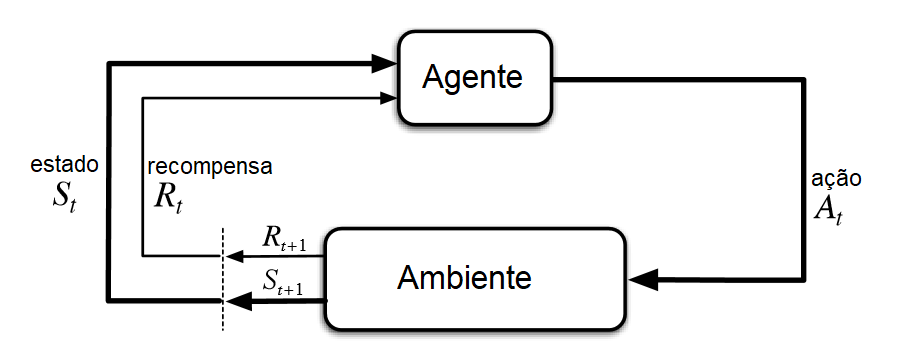
\includegraphics[width=0.60\textwidth]{fig/MDP.png}
 \caption{Exemplo de um Processo de Decisão de Markov (MDP).}
 \label{fig:mdp_ilustracao}
\end{figure}

Uma característica fundamental dos MDPs é a propriedade de Markov, que estabelece que a probabilidade de transição para um novo estado depende apenas do estado atual e da ação tomada, não dependendo de estados ou ações anteriores \cite{sutton}.

Os MDPs são amplamente utilizados em diversas áreas, incluindo:

\begin{itemize}
\item Robótica e controle automático
\item Planejamento de trajetórias
\item Gestão de recursos
\item Sistemas de recomendação
\item Jogos e simulações
\end{itemize}

Existem várias extensões dos MDPs para lidar com diferentes cenários:

\begin{itemize}
\item \textbf{POMDPs (Partially Observable MDPs)}: Lidam com situações onde o estado não é completamente observável.
\item \textbf{LLMDPs (Language-Limited MDPs)}: Incorporam restrições de linguagem nas ações e observações consideradas \cite{introducao_modelos_probabilisticos}.
\end{itemize}

Os MDPs fornecem uma base teórica sólida para o desenvolvimento de algoritmos de aprendizado por reforço, permitindo a modelagem e solução de problemas complexos de tomada de decisão sequencial sob incerteza.

\subsubsection{Funções de valor e política}
\label{subsubsec:valor_politica}

As funções de valor e política são conceitos fundamentais no aprendizado por reforço (RL), desempenhando papéis cruciais na tomada de decisões e na avaliação de estratégias. As funções de valor estimam o quão vantajoso é para um agente estar em um determinado estado ou executar uma ação específica em um estado. Existem dois tipos principais de funções de valor: a Função de Valor de Estado (V-function) e a Função de Valor de Ação (Q-function).

A Função de Valor de Estado, representada como \( V^\pi(s) \), indica o valor esperado de estar em um estado específico seguindo uma política \(\pi\). Matematicamente, é definida como \( V^\pi(s) = \mathbb{E}_\pi[G_t | S_t = s] \), onde \( G_t \) é o retorno acumulado a partir do tempo \( t \). Por outro lado, a Função de Valor de Ação, representada como \( Q^\pi(s,a) \), indica o valor esperado de tomar uma ação específica em um estado específico e depois seguir uma política \(\pi\). Sua definição matemática é \( Q^\pi(s,a) = \mathbb{E}_\pi[G_t | S_t = s, A_t = a] \).

Essas funções de valor são essenciais para métodos baseados em valor, como Q-learning e DQN (Deep Q-Network) \cite{ Liu2020OverviewOR}. Elas permitem que o agente avalie a qualidade das ações em diferentes estados, facilitando a tomada de decisões ótimas.

As funções de política, por sua vez, definem o comportamento do agente, mapeando estados para ações. Existem dois tipos principais de políticas: a Política Determinística e a Política Estocástica. A Política Determinística mapeia cada estado para uma única ação, representada como \(\pi(s) = a\). Já a Política Estocástica mapeia cada estado para uma distribuição de probabilidade sobre as ações, representada como \(\pi(a|s) = P(A_t = a | S_t = s)\).

As funções de política são centrais para métodos baseados em política, como Policy Gradient e PPO (Proximal Policy Optimization) \cite{ Liu2020OverviewOR}. Elas permitem que o agente aprenda diretamente qual ação tomar em cada estado, sem necessariamente estimar valores de estado ou ação.

A relação entre funções de valor e política é estreita. A função de valor avalia a qualidade de uma política, enquanto a política pode ser derivada da função de valor, por exemplo, escolhendo a ação com o maior valor \( Q \) em cada estado. Alguns métodos, como os algoritmos ator-crítico, combinam ambos os conceitos: o "ator" (política) decide quais ações tomar, e o "crítico" (função de valor) avalia essas ações e fornece feedback para melhorar a política \cite{ Liu2020OverviewOR}.

O objetivo do RL é encontrar a política ótima \(\pi^*\) que maximize o retorno esperado. Isso pode ser alcançado de várias maneiras: métodos baseados em valor aprendem a função de valor ótima e derivam a política ótima a partir dela \cite{ Takada2020ReinforcementLT}; métodos baseados em política otimizam diretamente a política, muitas vezes usando gradientes de política \cite{ Liu2020OverviewOR}; e métodos híbridos combinam aprendizado de valor e otimização de política, como em algoritmos ator-crítico \cite{ yao2020smixlambdaenhancingcentralizedvalue}.

Recentes avanços incluem o uso de redes neurais profundas para aproximar funções de valor e política em ambientes complexos, como demonstrado no jogo de Hex \cite{ Takada2020ReinforcementLT}, e o desenvolvimento de métodos robustos para lidar com incertezas e riscos em ambientes desafiadores \cite{ Kim_2022}.

As funções de valor e política são elementos cruciais no aprendizado por reforço (RL), especialmente em algoritmos avançados como o Proximal Policy Optimization (PPO). No PPO, as funções de valor são utilizadas para estimar a vantagem, que é essencial para o processo de otimização da política. A política, por sua vez, é ajustada para maximizar uma função objetivo surrogate, garantindo que as atualizações sejam estáveis e eficientes. Essa interação entre funções de valor e política permite que o PPO aprenda de forma eficaz em ambientes complexos, equilibrando desempenho e estabilidade. Vamos explorar esses conceitos e sua relação com o PPO.



\subsection{Aprendizado por Reforço Profundo}
\label{subsec:deep_rl}

O Aprendizado por Reforço Profundo (Deep Reinforcement Learning - DRL) é uma abordagem avançada de aprendizado de máquina que combina os princípios do aprendizado por reforço tradicional com as capacidades das redes neurais profundas. Esta técnica tem ganhado destaque significativo nos últimos anos devido à sua eficácia em resolver problemas complexos de tomada de decisão sequencial.

O Aprendizado por Reforço Profundo é um paradigma de aprendizado de máquina no qual um agente aprende a tomar decisões ótimas através da interação com um ambiente, utilizando redes neurais profundas para representar e processar informações complexas \cite{Job2023TelemetriaAU, Kinoshita2022AprendizadoPR}. O objetivo principal é maximizar uma recompensa cumulativa ao longo do tempo, permitindo que o agente aprenda políticas de ação eficazes em ambientes dinâmicos e de alta dimensionalidade.

Uma característica fundamental do DRL é o aprendizado baseado em experiência. O agente aprende através da interação direta com o ambiente, acumulando experiência ao longo do tempo \cite{Jesus2023AprendizadoPR, Grando2021AprendizadoPR}. As decisões são tomadas com base em um processo de tentativa e erro, onde o agente explora diferentes ações e aprende com os resultados obtidos.

Além disso, o DRL utiliza redes neurais profundas para processar e representar informações de alta dimensionalidade, como imagens ou dados sensoriais complexos \cite{Bezerra2021PropostaDC, Bezerra2023AprendizagemPR}. Isso permite a extração automática de características relevantes do ambiente, eliminando a necessidade de engenharia manual de recursos.

Outra característica importante é a adaptabilidade. O agente pode se adaptar a mudanças no ambiente e generalizar seu aprendizado para situações não vistas anteriormente \cite{Bezerra2021PropostaDC, Bezerra2023AprendizagemPR}. O DRL é capaz de lidar com problemas parcialmente observáveis, onde nem toda a informação sobre o estado do ambiente está disponível.

O DRL também foca na otimização de longo prazo, buscando maximizar a recompensa cumulativa ao longo do tempo, em vez de apenas recompensas imediatas \cite{Bezerra2021PropostaDC, Bezerra2023AprendizagemPR}. Isso permite o aprendizado de estratégias complexas que envolvem planejamento e tomada de decisão em múltiplos passos.

Um dos desafios do DRL é balancear a necessidade de explorar novas ações para descobrir melhores estratégias com a exploração de ações conhecidas que já produzem bons resultados \cite{Bezerra2021PropostaDC, Bezerra2023AprendizagemPR}. Técnicas como $\epsilon$-greedy ou amostragem de Thompson são utilizadas para gerenciar este trade-off.

O Aprendizado por Reforço Profundo tem sido aplicado com sucesso em diversas áreas, incluindo navegação autônoma de robôs e veículos \cite{Job2023TelemetriaAU, Kinoshita2022AprendizadoPR}, jogos eletrônicos e simulações complexas \cite{Jesus2023AprendizadoPR, Grando2021AprendizadoPR}, otimização de sistemas de controle industrial \cite{Bezerra2021PropostaDC, Bezerra2023AprendizagemPR}, negociação automatizada em mercados financeiros \cite{Bezerra2021PropostaDC, Bezerra2023AprendizagemPR}, e gerenciamento de redes de comunicação e IoT \cite{Bezerra2021PropostaDC, Bezerra2023AprendizagemPR}.

Apesar de seu potencial, o DRL também enfrenta desafios significativos, como alta demanda computacional e longo tempo de treinamento \cite{Job2023TelemetriaAU, Kinoshita2022AprendizadoPR}, dificuldade em transferir o aprendizado de ambientes simulados para o mundo real \cite{Jesus2023AprendizadoPR, Grando2021AprendizadoPR}, sensibilidade a hiperparâmetros e configurações de treinamento \cite{Bezerra2021PropostaDC, Bezerra2023AprendizagemPR}, e a necessidade de grandes quantidades de dados e interações para aprendizado efetivo \cite{Bezerra2021PropostaDC, Bezerra2023AprendizagemPR}.


\subsubsection{Redes neurais como aproximadores de função}
\label{subsubsec:redes_neurais}

As redes neurais como aproximadores de função desempenham um papel fundamental no contexto do Aprendizado por Reforço Profundo (DRL), representando uma das principais diferenças em relação ao aprendizado por reforço tradicional. Esta abordagem permite que os agentes de DRL lidem com espaços de estado e ação contínuos e de alta dimensionalidade, superando limitações significativas dos métodos tabulares convencionais.


No DRL, as redes neurais são utilizadas para aproximar funções complexas que mapeiam estados para valores (função de valor) ou ações (função de política). Essa capacidade de aproximação é crucial por várias razões:

1. \textbf{Generalização}: As redes neurais podem generalizar para estados não vistos anteriormente, interpolando ou extrapolando com base em padrões aprendidos.

2. \textbf{Compressão de Informação}: Permitem representar funções complexas de forma compacta, evitando a necessidade de armazenar valores para cada estado possível.

3. \textbf{Aprendizado de Características}: Extraem automaticamente características relevantes dos dados de entrada, eliminando a necessidade de engenharia manual de recursos.


\textbf{Aproximação da Função de Valor}: As redes neurais são utilizadas para estimar o valor esperado de estados ou pares estado-ação. Isso é particularmente útil em algoritmos como o Deep Q-Network (DQN), onde a rede neural aproxima a função Q, que representa o valor de longo prazo de tomar uma ação específica em um determinado estado.

\textbf{Aproximação da Função de Política}: Em métodos baseados em política, como o PPO (Proximal Policy Optimization), as redes neurais são usadas para representar diretamente a política do agente. Elas mapeiam estados para distribuições de probabilidade sobre ações, permitindo que o agente tome decisões em ambientes contínuos ou de alta dimensionalidade.

\textbf{Modelos de Ambiente}: Em algumas abordagens de DRL baseadas em modelo, as redes neurais são usadas para aproximar a dinâmica do ambiente, prevendo estados futuros e recompensas com base em estados e ações atuais.


As vantagens incluem a capacidade de lidar com espaços de estado e ação contínuos, a habilidade de processar entradas de alta dimensionalidade, como imagens ou dados sensoriais complexos, e o potencial para transferência de aprendizado entre tarefas similares. 

Os desafios envolvem a instabilidade de treinamento devido à não-estacionariedade do processo de aprendizagem, o overfitting em conjuntos de dados limitados, e a dificuldade em interpretar as decisões do modelo devido à natureza de "caixa preta" das redes neurais profundas.


No contexto do PPO, as redes neurais são utilizadas tanto para aproximar a função de política quanto para estimar a função de valor. A política é representada por uma rede neural que mapeia estados para distribuições de probabilidade sobre ações, enquanto uma segunda rede (ou uma rede compartilhada com saídas separadas) estima o valor de cada estado.

O uso de redes neurais como aproximadores de função no PPO permite que o algoritmo lide eficientemente com ambientes complexos e contínuos. A técnica de clipping do PPO, que limita as mudanças na política, ajuda a estabilizar o treinamento dessas redes neurais, mitigando alguns dos desafios associados à aproximação de função em DRL.


\subsection{Proximal Policy Optimization (PPO)}
\label{subsec:ppo}

\subsubsection{Motivação e princípios do PPO}
\label{subsubsec:ppo_principios}

O Proximal Policy Optimization (PPO) surgiu como uma resposta às limitações dos algoritmos de aprendizado por reforço anteriores, visando melhorar a estabilidade e eficiência do treinamento em ambientes complexos. O PPO foi desenvolvido para abordar os desafios de otimização de políticas em espaços de ação contínuos e de alta dimensionalidade, comuns em problemas do mundo real.

Os princípios fundamentais do PPO incluem:

1. Atualização conservadora de política: O PPO busca realizar atualizações de política que sejam significativas, mas não excessivamente grandes, para evitar colapsos de desempenho.

2. Equilíbrio entre exploração e aproveitamento: O algoritmo mantém um equilíbrio entre explorar novas ações e aproveitar as ações conhecidas que produzem bons resultados.

3. Eficiência amostral: O PPO é projetado para aprender de forma eficiente a partir de experiências limitadas, reduzindo a quantidade de dados necessários para o treinamento.

\subsubsection{Função objetivo e mecanismo de clipping}
\label{subsubsec:ppo_objetivo}

A função objetivo do PPO é projetada para incentivar melhorias na política enquanto evita mudanças drásticas. O componente central desta função é o mecanismo de clipping, que limita a magnitude das atualizações de política~\cite{Cheng2022AuthenticBoundary}.

A função objetivo do PPO pode ser expressa como:

\begin{equation}
L^{\text{CLIP}}(\theta) = \mathbb{E}_t[\min(r_t(\theta)\hat{A}_t, \text{clip}(r_t(\theta), 1-\epsilon, 1+\epsilon)\hat{A}_t)]
\end{equation}

Onde:

\begin{itemize}
    \item $r_t(\theta)$ é a razão entre a nova e a antiga probabilidade de ação
    \item $\hat{A}_t$ é a estimativa de vantagem
    \item $\epsilon$ é o parâmetro de clipping
\end{itemize}

O mecanismo de clipping garante que a razão de probabilidade $r_t(\theta)$ permaneça dentro de um intervalo $[1-\epsilon, 1+\epsilon]$, impedindo atualizações excessivamente grandes na política. Isso promove uma aprendizagem mais estável e reduz o risco de colapso de desempenho durante o treinamento~\cite{Jia2024ProximalPO}.

\subsubsection{Vantagens do PPO em ambientes contínuos e multiagentes}
\label{subsubsec:ppo_vantagens}

O PPO demonstra várias vantagens em ambientes contínuos e multiagentes:

1. Estabilidade em espaços de ação contínuos: O PPO é particularmente eficaz em problemas com espaços de ação contínuos, como controle robótico e navegação autônoma\cite{pendyala2024solvingrealworldoptimizationproblem,han2018amberadaptivemultibatchexperience}.

2. Escalabilidade para sistemas multiagentes: O algoritmo se adapta bem a cenários com múltiplos agentes, permitindo a coordenação eficiente em ambientes complexos\cite{Mller2023MultiAgentPP}.

3. Eficiência computacional: Comparado a métodos centralizados, o PPO oferece vantagens em termos de complexidade computacional, garantindo tempos de planejamento curtos em ambientes de larga escala \cite{Li2022ResearchOO}.

4. Adaptabilidade a diferentes números de agentes: Políticas aprendidas com PPO demonstram boa escalabilidade, podendo ser aplicadas a diferentes números de agentes sem perda significativa de desempenho\cite{Mller2023MultiAgentPP}.

5. Robustez em tarefas de longo prazo: O PPO é capaz de lidar com recompensas extremamente atrasadas e horizontes de tempo longos, tornando-o adequado para tarefas complexas do mundo real\cite{pendyala2024solvingrealworldoptimizationproblem}.

6. Flexibilidade na engenharia de recompensas: O PPO permite a incorporação de mecanismos sofisticados de recompensa, como recompensas de densidade e penalidades de etapas, para melhorar a eficiência da tarefa e reduzir comportamentos indesejados\cite{Li2022ResearchOO}.

Essas vantagens tornam o PPO uma escolha popular para uma ampla gama de aplicações, desde jogos e robótica até sistemas de transporte e otimização de processos industriais\cite{pendyala2024solvingrealworldoptimizationproblem,Tiong2022AutonomousVP,Mller2023MultiAgentPP}.
%% - - - - - - - - - - - - - - - - - - - - - - - - - - - - - - - - - - -
\section{Aprendizado por Reforço Multiagente}
\label{sec:marl}

No contexto de aprendizado por reforço (reinforcement learning) e aprendizado por reforço profundo (deep reinforcement learning), vamos detalhar os conceitos solicitados:

O Aprendizado por Reforço Multiagente (Multi-Agent Reinforcement Learning - MARL) é uma extensão do aprendizado por reforço tradicional que lida com ambientes onde múltiplos agentes interagem simultaneamente\cite{azadeh2024advancesmultiagentreinforcementlearning,baheri2024synergyoptimaltransporttheory}. Nesse cenário, os agentes devem aprender a tomar decisões ótimas considerando não apenas o ambiente, mas também as ações e estratégias dos outros agentes.

No MARL, cada agente busca maximizar sua própria recompensa, mas suas ações afetam o ambiente compartilhado e, consequentemente, as recompensas dos outros agentes\cite{Li2023RACEIM,wang2024multipleshipscooperativenavigation}. Isso cria um cenário complexo onde a cooperação e a competição entre agentes desempenham papéis cruciais.

\subsection{Desafios em Ambientes Multiagente}
\label{subsec:desafios_multi}

\subsubsection{Coordenação e competição entre agentes}
\label{subsubsec:coordenacao}

A coordenação e competição entre agentes são aspectos fundamentais do MARL que apresentam desafios significativos:

1. Coordenação: Em cenários cooperativos, os agentes precisam aprender a trabalhar juntos para atingir objetivos comuns\cite{Li2023RACEIM}. Isso envolve:
   - Desenvolvimento de estratégias conjuntas
   - Compartilhamento de informações relevantes
   - Sincronização de ações para maximizar a eficiência coletiva

2. Competição: Em ambientes competitivos ou mistos, os agentes podem ter objetivos conflitantes\cite{baheri2024synergyoptimaltransporttheory}. Isso leva a:
   - Necessidade de prever e reagir às ações dos oponentes
   - Desenvolvimento de estratégias robustas contra adversários adaptativos
   - Equilíbrio entre cooperação e competição em cenários mistos

Para lidar com esses desafios, técnicas como o uso de métricas de alinhamento de políticas baseadas na distância de Wasserstein têm sido propostas para melhorar a coordenação entre agentes\cite{Li2023RACEIM}.

\subsubsection{Não-estacionariedade do ambiente}
\label{subsubsec:nao_estacionariedade}

A não-estacionariedade é um dos principais desafios em MARL e refere-se à mudança constante do ambiente do ponto de vista de cada agente individual\cite{NiedzikaDomaski2024AnEM,delafuente2024gametheorymultiagentreinforcement}. Isso ocorre porque:

1. Agentes em evolução: Cada agente está continuamente aprendendo e adaptando suas políticas, o que altera o ambiente para os outros agentes\cite{NiedzikaDomaski2024AnEM}.

2. Dinâmica complexa: As interações entre múltiplos agentes criam uma dinâmica que é difícil de prever e modelar\cite{delafuente2024gametheorymultiagentreinforcement}.

3. Observações parciais: Muitas vezes, os agentes têm acesso apenas a informações locais, o que dificulta a compreensão completa do estado do ambiente\cite{NiedzikaDomaski2024AnEM}.

A não-estacionariedade apresenta vários desafios:

- Instabilidade na aprendizagem: As políticas que eram ótimas em um momento podem se tornar subótimas rapidamente.
- Exploração ineficiente: Estratégias de exploração eficazes em ambientes estacionários podem falhar em ambientes não-estacionários.
- Convergência difícil: A constante mudança no ambiente pode impedir que os agentes convirjam para políticas estáveis.

Para abordar a não-estacionariedade, pesquisadores têm proposto várias soluções:

- Uso de modelos do ambiente para prever mudanças e adaptar as políticas dos agentes\cite{NiedzikaDomaski2024AnEM}.
- Desenvolvimento de algoritmos que consideram explicitamente a natureza não-estacionária do ambiente, como variantes do algoritmo MADDPG (Multi-Agent Deep Deterministic Policy Gradient)\cite{Li2023RACEIM}.
- Implementação de técnicas de comunicação entre agentes para melhorar a coordenação e adaptação às mudanças do ambiente\cite{Li2023RACEIM}.

Essas abordagens visam melhorar a robustez e a eficácia dos sistemas de MARL em ambientes complexos e dinâmicos, permitindo que os agentes aprendam e se adaptem de forma mais eficiente em cenários multiagente desafiadores.

% \subsection{Aplicações em Futebol de Robôs}
% \label{subsec:futebol_robos}

% \subsubsection{Visão geral da categoria SSL-EL}
% \label{subsubsec:ssl_el}

% \subsubsection{Desafios específicos do domínio}
% \label{subsubsec:desafios_dominio}

%% - - - - - - - - - - - - - - - - - - - - - - - - - - - - - - - - - - -
\section{Técnicas de Aprendizado Progressivo}
\label{sec:aprendizado_prog}

No contexto de aprendizado por reforço (reinforcement learning) e aprendizado por reforço profundo (deep reinforcement learning), as técnicas de aprendizado progressivo são abordagens que visam melhorar a eficiência e eficácia do processo de aprendizagem dos agentes. O aprendizado progressivo, também conhecido como aprendizado incremental ou currículo de aprendizagem, é uma estratégia que facilita o aprendizado de tarefas complexas dividindo-as em subtarefas mais simples e gradualmente aumentando a dificuldade. Os princípios fundamentais dessa técnica incluem a decomposição de tarefas, onde o problema principal é dividido em subtarefas mais gerenciáveis, o sequenciamento, que organiza as subtarefas em uma ordem crescente de complexidade, e a transferência de conhecimento, onde o aprendizado adquirido em tarefas mais simples é utilizado como base para tarefas mais complexas. 

Implementações em RL e Deep RL incluem o currículo de aprendizagem, que inicia o treinamento com versões simplificadas do ambiente e gradualmente aumenta a complexidade à medida que o agente melhora seu desempenho, o aprendizado hierárquico, que utiliza uma estrutura hierárquica de políticas onde políticas de alto nível selecionam subtarefas e políticas de baixo nível executam ações específicas, a transferência de aprendizado, onde o conhecimento adquirido em tarefas similares é transferido para acelerar o aprendizado em novas tarefas, e o meta-aprendizado, onde o agente aprende a aprender, desenvolvendo estratégias gerais que podem ser rapidamente adaptadas a novas situações. Os benefícios dessas técnicas incluem um aprendizado mais rápido, melhor generalização, superação de mínimos locais e escalabilidade, permitindo abordar problemas mais complexos que seriam intratáveis com abordagens diretas. No entanto, desafios como o design do currículo, o equilíbrio entre exploração e aproveitamento, e a necessidade de evitar overfitting são aspectos críticos a serem considerados. As técnicas de aprendizado progressivo representam uma área promissora na pesquisa de RL e Deep RL, oferecendo caminhos para superar limitações tradicionais e abordar problemas cada vez mais complexos do mundo real\cite{DeSouzaRibeiro2024AuxlioAD,Brito2023AplicaesDA,Felippe2024OUD,Rocha2024SonsPE,Dias2023AplicaoDA,Geremias2024OUD}.

\subsection{Curriculum Learning}
\label{subsec:curriculum}

Curriculum Learning é uma abordagem de aprendizado progressivo inspirada na forma como os seres humanos aprendem, começando com conceitos simples e gradualmente progredindo para tarefas mais complexas. A motivação por trás dessa técnica é melhorar a eficiência e eficácia do processo de aprendizagem em ambientes de Reinforcement Learning (RL) e Deep Reinforcement Learning (Deep RL). Os princípios fundamentais do Curriculum Learning incluem a ordenação de tarefas do mais fácil ao mais difícil, o aprendizado gradual expondo o agente a desafios progressivamente mais complexos e a transferência de conhecimento de tarefas simples para problemas mais elaborados.

\subsubsection{Conceito e motivação}
\label{subsubsec:curriculum_conceito}

O conceito de Curriculum Learning baseia-se na ideia de que a aprendizagem pode ser facilitada ao estruturar o processo de ensino de maneira incremental. Isso significa que, ao invés de expor o agente a tarefas complexas desde o início, ele é inicialmente treinado em tarefas mais simples, que são gradualmente substituídas por tarefas mais difíceis à medida que o agente adquire habilidades e conhecimento. A motivação para essa abordagem é que ela pode levar a um aprendizado mais eficiente e eficaz, permitindo que o agente desenvolva uma base sólida de conhecimento antes de enfrentar desafios mais complexos. Essa técnica é particularmente útil em ambientes de RL e Deep RL, onde a complexidade das tarefas pode variar significativamente e a capacidade de transferir conhecimento de tarefas simples para problemas mais elaborados pode ser crucial para o sucesso do agente.

\subsubsection{Desenho de currículos para RL}
\label{subsubsec:curriculum_desenho}

O desenho de currículos eficazes para RL é um aspecto crucial do Curriculum Learning. Algumas estratégias incluem a modificação do ambiente, onde inicialmente o agente interage com versões simplificadas do ambiente, com a complexidade aumentando gradualmente. Outra estratégia é a seleção de tarefas, onde um algoritmo seleciona tarefas apropriadas baseadas no nível atual de habilidade do agente. Além disso, a estrutura de recompensas pode ser ajustada ao longo do tempo, começando com recompensas mais frequentes para comportamentos básicos e progredindo para recompensas mais esparsas focadas em comportamentos complexos. O design eficaz de um currículo frequentemente requer conhecimento especializado do domínio, e a automatização desse processo é uma área ativa de pesquisa\cite{Sukhbaatar2018learninggoalembeddingsselfplay}.

\subsubsection{Aplicações em robótica e jogos}
\label{subsubsec:curriculum_aplicacoes}

Curriculum Learning tem demonstrado resultados promissores em diversas aplicações, incluindo robótica e jogos. Em manipuladores robóticos, o Curriculum Learning tem sido aplicado para melhorar o aprendizado de tarefas complexas. Técnicas como Q-Learning, Deep Reinforcement Learning, Actor-Critic e Policy Gradient são frequentemente utilizadas nesse contexto\cite{Brito2023AplicaesDA}. No campo dos jogos digitais educacionais, abordagens de aprendizado progressivo, como o Curriculum Learning, podem ser integradas com Game Learning Analytics para melhorar a experiência de aprendizado e o engajamento dos jogadores\cite{Geremias2024OUD}. Além disso, estudos têm aplicado Curriculum Learning em experimentos de navegação autônoma, demonstrando como variações nos parâmetros de aprendizado, como taxa de aprendizado e fator de desconto, podem afetar significativamente o desempenho do agente\cite{Sukhbaatar2018learninggoalembeddingsselfplay}. O Curriculum Learning oferece benefícios significativos, incluindo aprendizado mais rápido, melhor generalização e superação de mínimos locais. No entanto, desafios como o design adequado do currículo e o balanceamento entre tarefas fáceis e difíceis permanecem áreas de pesquisa ativa no campo de RL e Deep RL.

\subsection{Self-Play}
\label{subsec:self_play}

\subsubsection{Princípios do self-play em RL}
\label{subsubsec:self_play_principios}

O self-play em RL baseia-se no princípio de que um agente pode aprender e melhorar suas habilidades jogando contra si mesmo. Este método envolve aspectos fundamentais como o aprendizado simétrico, onde o agente assume ambos os papéis em um ambiente competitivo, aprendendo estratégias tanto ofensivas quanto defensivas\cite{Sukhbaatar2018learninggoalembeddingsselfplay}. Além disso, o self-play permite a geração de uma grande quantidade de dados de treinamento sem a necessidade de oponentes externos ou humanos\cite{Sukhbaatar2018learninggoalembeddingsselfplay}.

Ao jogar contra versões anteriores de si mesmo, o agente explora continuamente novas estratégias e contra-estratégias\cite{Sukhbaatar2018learninggoalembeddingsselfplay}, adaptando-se constantemente às suas próprias melhores estratégias em um processo de melhoria contínua\cite{Sukhbaatar2018learninggoalembeddingsselfplay}. Através do self-play, os agentes podem desenvolver habilidades que generalizam bem para novos cenários ou oponentes não vistos durante o treinamento\cite{Sukhbaatar2018learninggoalembeddingsselfplay}.

\subsubsection{Exemplos de sucesso em jogos complexos}
\label{subsubsec:self_play_exemplos}

O self-play tem demonstrado resultados impressionantes em diversos jogos complexos. No jogo de Go, o AlphaGo e suas iterações posteriores utilizaram self-play para alcançar e superar o nível de jogadores humanos profissionais\cite{Sukhbaatar2018learninggoalembeddingsselfplay}. No xadrez, programas baseados em deep reinforcement learning e self-play, como o AlphaZero, alcançaram níveis sobre-humanos\cite{Sukhbaatar2018learninggoalembeddingsselfplay}.

Em jogos ainda mais complexos, como Starcraft II, agentes treinados com self-play conseguiram competir em alto nível\cite{Sukhbaatar2018learninggoalembeddingsselfplay}. No Dota 2, o OpenAI Five demonstrou habilidades competitivas contra equipes profissionais\cite{Sukhbaatar2018learninggoalembeddingsselfplay}. No poker, agentes de IA treinados com self-play alcançaram níveis sobre-humanos em variantes com múltiplos jogadores\cite{Sukhbaatar2018learninggoalembeddingsselfplay}.

No contexto do futebol de robôs, o self-play tem demonstrado resultados significativos no desenvolvimento de habilidades complexas e coordenação multiagente. Por exemplo, robôs têm sido treinados para realizar movimentos sofisticados como recuperação de quedas, caminhada, giros e chutes através do self-play em ambientes simulados\cite{Brando2022MultiagentRL}. A técnica também tem se mostrado eficaz no treinamento de equipes para cooperação e competição simultânea, permitindo que os robôs aprendam a se adaptar a situações de jogo dinâmicas e desenvolvam estratégias que generalizam bem contra novos oponentes\cite{Brando2022MultiagentRL}. Além disso, o self-play tem sido aplicado com sucesso no desenvolvimento de sistemas completamente autônomos capazes de lidar com observações parciais do ambiente, simulando as imperfeições de sistemas de visão reais\cite{Szemenyei2020LearningTP}.



%\subsubsection{Geração automática de currículos via self-play}
%\label{subsubsec:self_play_curriculos}



%% - - - - - - - - - - - - - - - - - - - - - - - - - - - - - - - - - - -
% \section{Integração de Técnicas para Aquisição Progressiva de Habilidades}
% \label{sec:integracao}

% \subsection{Combinando Curriculum Learning e Self-Play}
% \label{subsec:combinacao}

% \subsubsection{Sinergias entre as abordagens}
% \label{subsubsec:sinergias}

% \subsubsection{Desafios na integração}
% \label{subsubsec:desafios_integracao}

% \subsection{Aplicação ao Futebol de Robôs Multiagente}
% \label{subsec:aplicacao_futebol}

% \subsubsection{Desenho de currículos para habilidades de futebol}
% \label{subsubsec:curriculos_futebol}

% \subsubsection{Transição do curriculum para self-play competitivo}
% \label{subsubsec:transicao_self_play}

% \subsubsection{Potenciais benefícios na aquisição de habilidades complexas}
% \label{subsubsec:beneficios_aquisicao}